\documentclass[review]{elsarticle}
\usepackage{comment}
\usepackage{url}
%
\usepackage[breaklinks]{hyperref}
\usepackage{breakurl}


\usepackage[ruled]{algorithm2e}

%\usepackage{lineno}
%\modulolinenumbers[5]

\journal{Optics Communications}

%%%%%%%%%%%%%%%%%%%%%%%
%% Elsevier bibliography styles
%%%%%%%%%%%%%%%%%%%%%%%
%% To change the style, put a % in front of the second line of the current style and
%% remove the % from the second line of the style you would like to use.
%%%%%%%%%%%%%%%%%%%%%%%

%% Numbered
%\bibliographystyle{model1-num-names}

%% Numbered without titles
%\bibliographystyle{model1a-num-names}

%% Harvard
%\bibliographystyle{model2-names.bst}\biboptions{authoryear}

%% Vancouver numbered
%\usepackage{numcompress}\bibliographystyle{model3-num-names}

%% Vancouver name/year
%\usepackage{numcompress}\bibliographystyle{model4-names}\biboptions{authoryear}

%% APA style
%\bibliographystyle{model5-names}\biboptions{authoryear}

%% AMA style
%\usepackage{numcompress}\bibliographystyle{model6-num-names}

%% `Elsevier LaTeX' style
\bibliographystyle{elsarticle-num}
%%%%%%%%%%%%%%%%%%%%%%%
\usepackage{graphicx}
\usepackage{subcaption}
%%%%%%%%%%%%%%%%%%%%%%%%%%%%%%%%%%%%%%%%%%%%%%%%%%%%%%%%%%%%%%%%%%%%%%%%%%%%%%%%%%

\usepackage[svgnames]{xcolor} % Enabling colors by their 'svgnames'

\usepackage{amsmath}
\usepackage{amsfonts}
\usepackage{amssymb}
%%%%%%%%%%%%%%%%%%%%%%%%%%%%%%%%%%%%%%%%%%%%%%%%%%%%%%%%%%%%%%%%%%%%%%%%%%%%%%%%%%

 
\begin{document} 

\begin{frontmatter}

\title{Importance of Sampling Frequency in the Dynamic Speckle Analysis}
%\tnotetext[mytitlenote]{Fully documented templates are available in the 
%elsarticle package on \href{http://www.ctan.org/tex-archive/macros/latex/contrib/elsarticle}{CTAN}.}



% Group authors per affiliation:
\author{------ ----- -----}
\author{------ ----- -----}



\address{University Federal of Lavras, Lavras, Brazil}
\fntext[myfootnote2]{201518201@posgrad.ufla.br}
\fntext[myfootnote1]{robertobraga@deg.ufla.br }
% 


\begin{abstract}
In this article, we show as the variation of sampling frequency, 
in a dynamic speckle analysis, affect the value of some dynamic speckle index, 
in this case: the absolute value of the differences ($AVD$) index, the temporal 
speckle standard deviation index and the temporal 
speckle mean index.
we show that  the dynamic speckle index value decrease your maximum excursion with 
the grow of sampling frequency because this affect directly the time integration 
(exposition time) of camera.
\end{abstract}

\begin{keyword}
Frequency sampling \sep
Dynamic speckle index \sep 
Dynamic speckle index \sep 
Dynamic speckle analysis
\end{keyword}

\end{frontmatter}

\linenumbers

%%%%%%%%%%%%%%%%%%%%%%%%%%%%%%%%%%%%%%%%%%%%%%%%%%%%%%%%%%%%%%%%%%%%%%%%%%%%%%%%%%%%%%%%%
%%%%%%%%%%%%%%%%%%%%%%%%%%%%%%%%%%%%%%%%%%%%%%%%%%%%%%%%%%%%%%%%%%%%%%%%%%%%%%%%%%%%%%%%%
\section{Introduction}
Dynamic laser speckle is a phenomenon that is 
%%%%%%%%%%%%%%%%%%%%%%%%%%%%%%%%%%%%%%%%%%%%%%%%%%%%%%%%%%%%%%%%%%%%%%%%%%%%%%%%%%%%%%%%%
%%%%%%%%%%%%%%%%%%%%%%%%%%%%%%%%%%%%%%%%%%%%%%%%%%%%%%%%%%%%%%%%%%%%%%%%%%%%%%%%%%%%%%%%%
\section{System description}
\label{sec:description}




\subsection{Exposure time of the camera}
\label{subsec:expositiontime}
The acquisition time,  frame per seconds ($fps$) or sampling frequency ($F_s$), 
in the camera Marlin F-033 will be calculated in the 
 Table \ref{table:1}, where we can see, the shutter register value ($Shutter$), 
time base register value ($Base$),
exposure time ($Exposure$),
exposure time offset ($Offset$) and
effective exposure time ($E$); so that 
\begin{equation}
Exposure= Shutter \times Base,
\end{equation}
\begin{equation}
\frac{1}{F_s}=E= Exposure + Offset.
\end{equation}
Where,  $F_s$ is calculated in relation to the  $E$; being that,
the $Exposure$ represent the photography integration time and $E$ the effective time
between photographs.
\begin{table}[h!]
\centering
\begin{tabular}{||c c c c c||} 
 \hline
 $Shutter$ &  $Base$ [$\mu s$] & $Offset$ [$\mu s$] & $E$ [$ms$] & $F_s$ [$fps$]\\ [0.5ex] 
 \hline\hline
 3332  & 20  & 12  & 66.652  & 15.003  \\ 
 1665  & 20  & 12  & 33.312  & 30.019  \\ 
 1110  & 20  & 12  & 22.212  & 45.021  \\ 
 832   & 20  & 12  & 16.652  & 60.053  \\ [1ex] 
 \hline
\end{tabular}
\caption{Exposition time and sampling frequency}
\label{table:1}
\end{table}

\subsection{Data packages in the ink drying process}
\label{subsec:data1}
 This data package analyze a drying ink process, 
 where images data packages are taken at the times
 $\{0,$ $1,$ $2,$ $3,$ $4,$ $5,$ $6,$ $7,$ $8,$ $9,$ $10\}$ min. 
 In each time, the package
 has 512 images of 147 pixels of height and 166 pixels of width.
 They were use 4 different sampling frequency to the images in each package,
 being these frequencies $15$, $30$, $45$ and $60$ hz.

\subsection{Data package of the activity analysis in corn seed}
\label{subsec:data2}
 This data package analyze the activity of a corn seed with 3 days of germination. 
 In this point, 
 They are taken 4 image data packages with different sampling frequencies to each package,
 being these frequencies $15$, $30$, $45$ and $60$ hz.
 Each package has 512 images of 29 pixels of height and 31 pixels of width.
 

\subsection{Test 1: ink drying process}
\label{subsec:test1}
The Fig. \ref{fig:test1} represents the data analysis method, acquired at a 
sampling frequency of $F_s$, 
with the characteristic seen in the Section \ref{subsec:data1},
\begin{figure}[ht!]
\centering
\includegraphics[width=0.55\columnwidth]{test1.eps}
\caption{Data analysis of the ink drying process test.}
\label{fig:test1}
\end{figure}
where, $P(t)$ is an image data package at the time $t$ minutes.
The $MEAN$ block represent the calculus of a temporal speckle mean index from 
the package $P(t)$, returning the value $MEAN(t)$, as exposed in the Section \ref{sec:mean}. 
The $AVD$ block represent the calculus of a absolute values of the differences index from 
the package $P(t)$, returning the value $AVD(t)$, as exposed in the Section \ref{sec:avd}. 
The $STD$ block represent the calculus of a temporal speckle standard deviation index from 
the package $P(t)$, returning the value $STD(t)$, as exposed in the Section \ref{sec:std}.
And finally,
the block $HPF$ represents a digital finite impulse response ``high-pass filter'' 
with order $40$ and cut-off at $0.25F_s$ that causes to have the at end of path
the $STDF(t)$ index value, a frequency filtered version of $STD(t)$.
According the information of the data packages, 
we will have indexes values, for each minutes during 10 minutes.

\subsection{Test 2: Activity analysis in corn seed}
\label{subsec:test2}
The activity analysis of a corn seed, 
uses the information of data package seen in the Section \ref{subsec:data1}.
We analyze this information of similar way to the seen in the Section \ref{subsec:test1},
with the difference that is taken an data package at the time $t$ (3 days of germination). 


%%%%%%%%%%%%%%%%%%%%%%%%%%%%%%%%%%%%%%%%%%%%%%%%%%%%%%%%%%%%%%%%%%%%%%%%%%%%%%%%%%%%%%%%%
%%%%%%%%%%%%%%%%%%%%%%%%%%%%%%%%%%%%%%%%%%%%%%%%%%%%%%%%%%%%%%%%%%%%%%%%%%%%%%%%%%%%%%%%%
\section{Theoretical definitions}
\label{sec:theoretical}

\subsection{temporal speckle mean index}
\label{sec:mean}

\subsection{Absolute Values of the Differences (AVD)}
\label{sec:avd}
%% Following the working flow in Fig. 2, the randomly-selected points in the ROI were 
%% analysed, with respect to their behaviour in time, by means of the Absolute Values 
%% of the Differences (AVD) method [35] using the data in the COM without 
%% normalization. The AVD method can be expressed by Equation (1):

%% where the COM is the Co-Occurrence Matrix related to the THSP, and the i and j 
%% variables represent the line i and the column j of each point of the COM matrix.

Frequency composition from $F_s/4$ until $F_s/2$ Hz like as  $HPF$ of first order.


\subsection{Temporal speckle standard deviation index}
\label{sec:std}
Frequency composition from $0$ until $F_s/2$ Hz like as  $HPF$ of first order.

\subsection{Filtered temporal speckle standard deviation index}
\label{sec:stdf}
Frequency composition from $0$ until $F_s/2$ Hz like as  $HPF$ of first order.

%%%%%%%%%%%%%%%%%%%%%%%%%%%%%%%%%%%%%%%%%%%%%%%%%%%%%%%%%%%%%%%%%%%%%%%%%%%%%%%%%%%%%%%%%
%%%%%%%%%%%%%%%%%%%%%%%%%%%%%%%%%%%%%%%%%%%%%%%%%%%%%%%%%%%%%%%%%%%%%%%%%%%%%%%%%%%%%%%%%

\section{Numerical results} 
\label{sec:numericalresults}

\subsection{Result of test 1}
\label{subsec:resulttest1}
This test shows the analyze result of an ink drying process, across 10 minutes,
with the sampling frequency: $15$, $30$, $45$ and $60$Hz.

%%%%%%%%%%%%%%%%%%%%%%%%%%%%%%%%%%%%%%%%%%%%%%%%%%%%%%%%%%%%%%%%%%%%%%%%%%%%%%%%
The Figure \ref{fig:MEANtest1} analyze the $MEAN(t)$ index,
in the test showed in the Section \ref{subsec:test1},
to each time $t$ for 4 sampling frequencies.
\begin{figure}[ht!]
    \centering
    \includegraphics[width=0.5\textwidth]{FPS_f11_rawMEAN.eps}
    \caption{$MEAN$ index value.}\label{fig:MEANtest1}
\end{figure}
It easy to see as the value of index has a monotonous 
behavior over time. By other side the values in the curves decreases in proportion with 
the grow of sampling frequency.

%%%%%%%%%%%%%%%%%%%%%%%%%%%%%%%%%%%%%%%%%%%%%%%%%%%%%%%%%%%%%%%%%%%%%%%%%%%%%%%%
The Figure \ref{fig:AVDtest1} shows the result of analysis explained in the 
Section \ref{subsec:test1} about the $AVD(t)$ index.
\begin{figure}[ht!]
    \centering
    \begin{subfigure}{0.48\textwidth}
        \caption{$AVD$ index value.}
        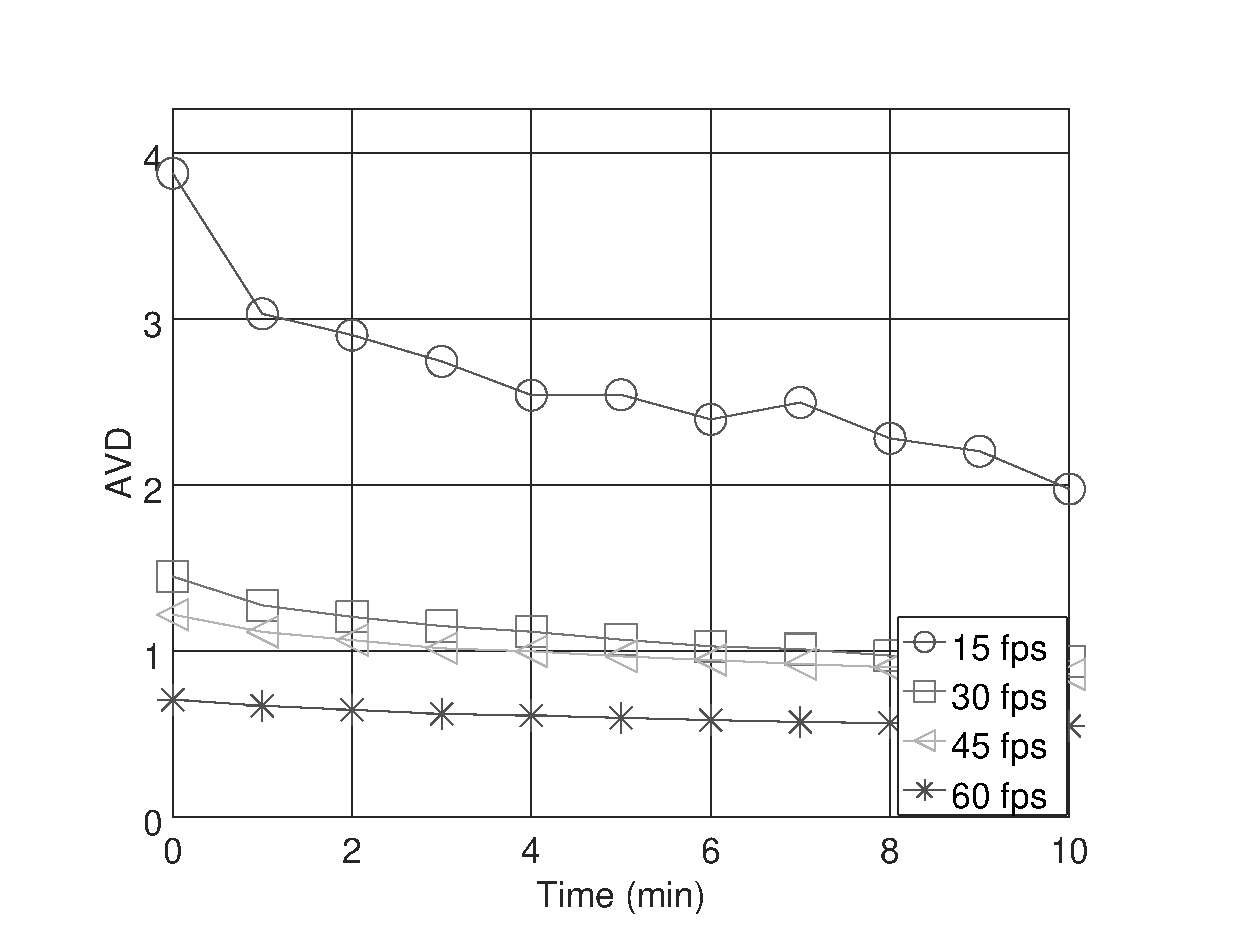
\includegraphics[width=\textwidth]{FPS_f11_rawAVD.eps}
        \label{fig:avdraw}
    \end{subfigure}
    ~ %add desired spacing between images, e. g. ~, \quad, \qquad, \hfill etc. 
      %(or a blank line to force the subfigure onto a new line)
    \begin{subfigure}{0.48\textwidth}
        \caption{Normalized $AVD$ index value.}
        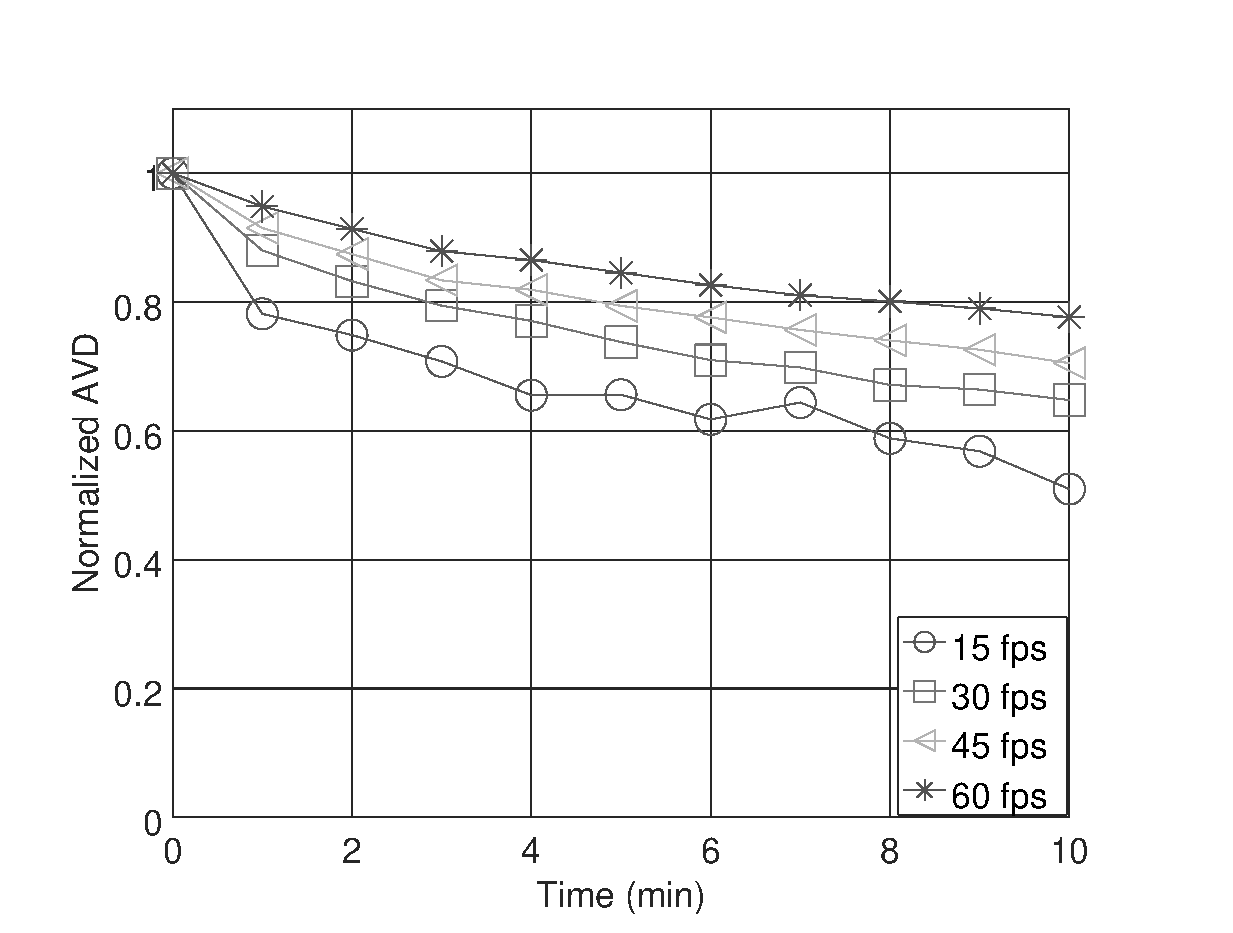
\includegraphics[width=\textwidth]{FPS_f11_norm1AVD.eps}
        \label{fig:avdnorm}
    \end{subfigure}
    \caption{$AVD$ index anaysis.}\label{fig:AVDtest1}
\end{figure}
The Figure \ref{fig:avdraw} shows the $AVD(t)$ index, in each time $t$, 
to 4 sampling frequencies, showing a different behavior across time in each sampling frequency,
so that, the value of the index in all  the curve decreases in proportion with 
the grow of sampling frequency. By other side,
the Figure \ref{fig:avdnorm} shows a normalized version of $AVD(t)$ index, 
so that the maximum value of curves have an unit value; thus,
It is easy to see that the maximum excursion of the curve is greater when decrease
the sampling frequency. Remembering that this index use information in a frequency
band between $F_s/4$ until $F_s/2$ Hz, as seen in Section \ref{sec:avd}.

%%%%%%%%%%%%%%%%%%%%%%%%%%%%%%%%%%%%%%%%%%%%%%%%%%%%%%%%%%%%%%%%%%%%%%%%%%%%%%%%
The Figure \ref{fig:STDtest1} analyze the $STD(t)$ index in the test showed in the 
Section \ref{subsec:test1}.
\begin{figure}[ht!]
    \centering
    \begin{subfigure}{0.48\textwidth}
        \caption{$STD$ index value.}
        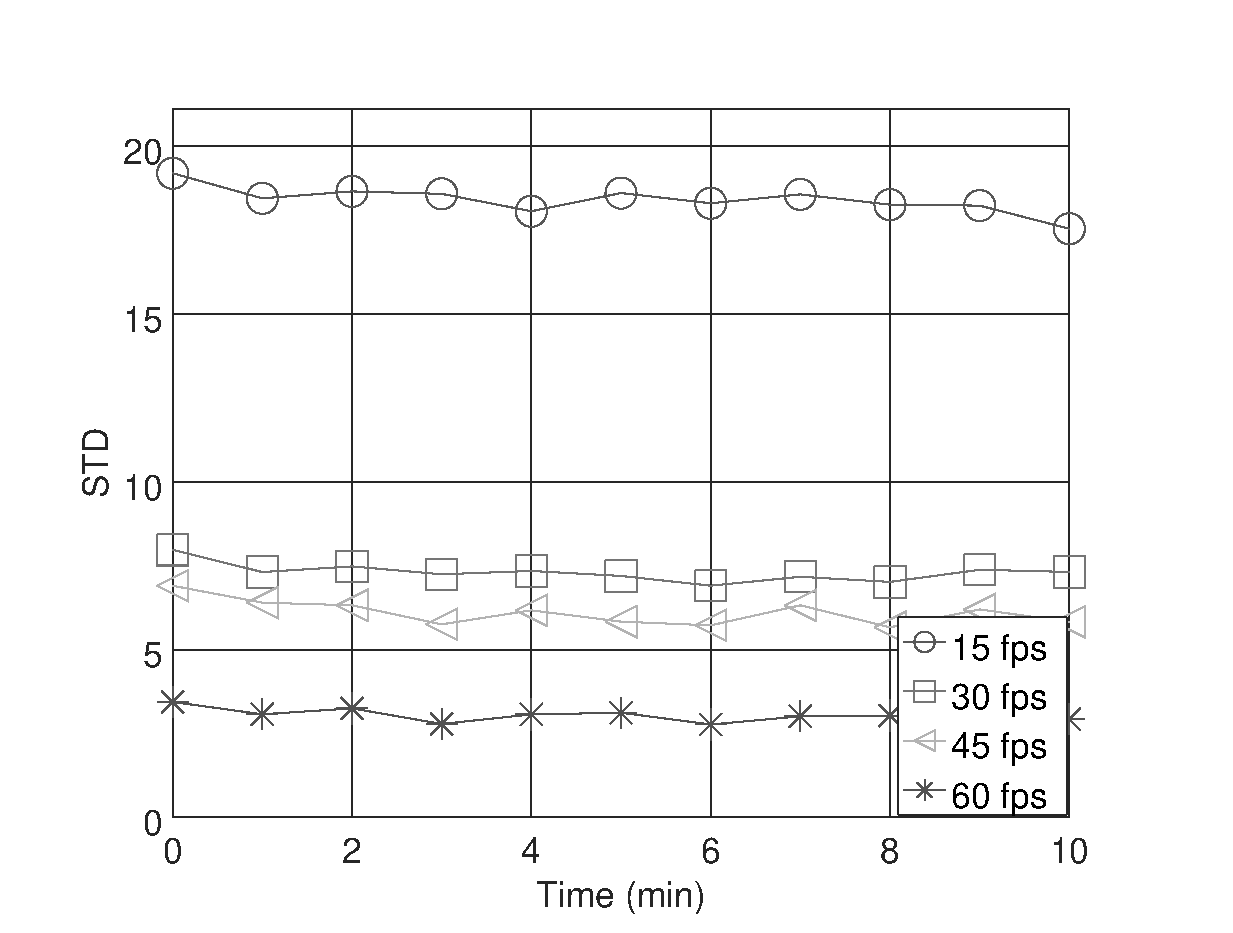
\includegraphics[width=\textwidth]{FPS_f11_rawSTD.eps}
        \label{fig:stdraw}
    \end{subfigure}
    ~ %add desired spacing between images, e. g. ~, \quad, \qquad, \hfill etc. 
      %(or a blank line to force the subfigure onto a new line)
    \begin{subfigure}{0.48\textwidth}
        \caption{Normalized $STD$ index value.}
        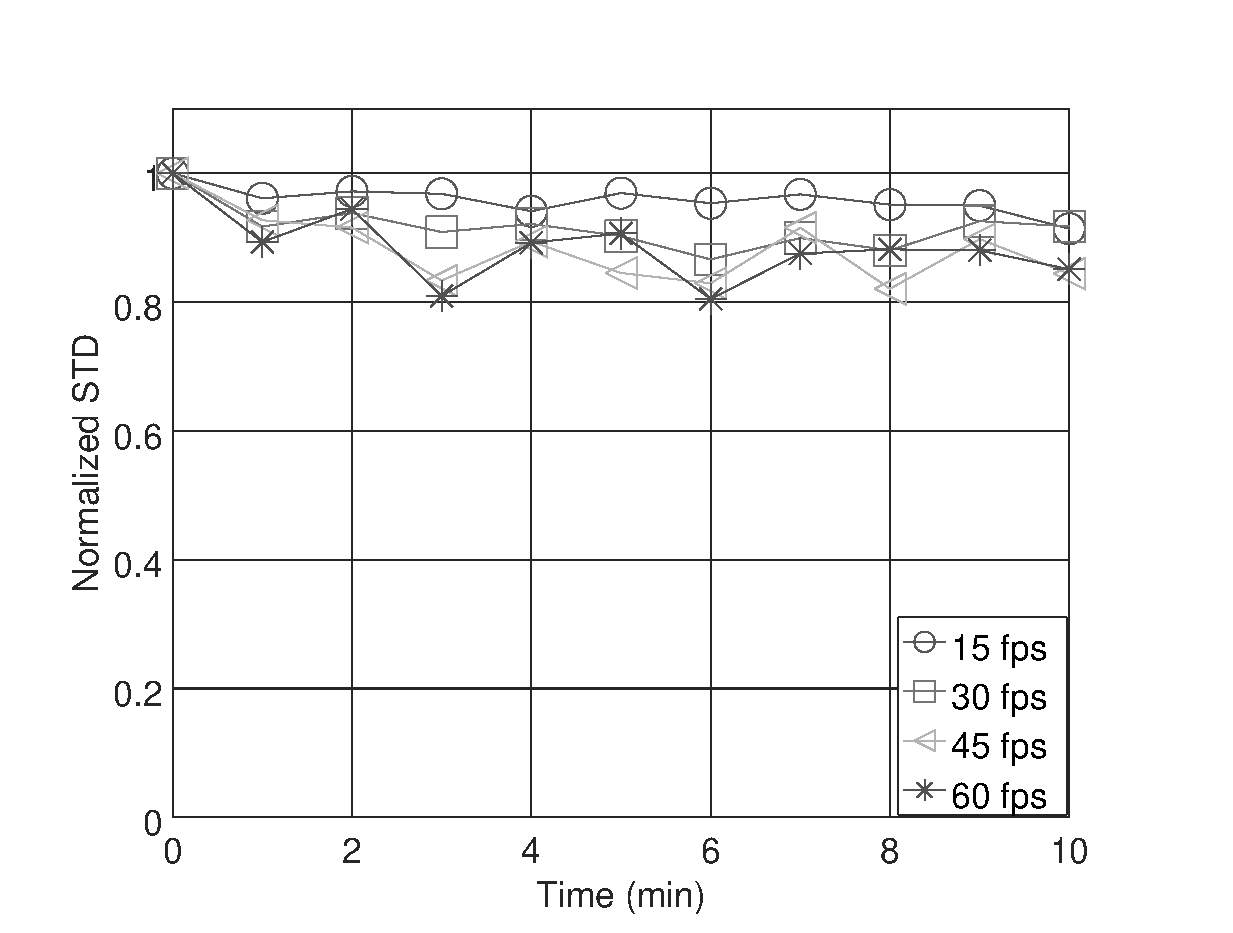
\includegraphics[width=\textwidth]{FPS_f11_norm1STD.eps}
        \label{fig:stdnorm}
    \end{subfigure}
    \caption{$STD$ index anaysis.}\label{fig:STDtest1}
\end{figure}
The Figure \ref{fig:stdraw} shows the  behavior of $STD(t)$ index, in each time $t$, 
to 4 different sampling frequencies. Remembering that this index uses information in a frequency
band between $0$ until $F_s/2$ Hz, as seen in Section \ref{sec:std}.
This index shows a different behavior across time to each sampling frequency,
so that, the value of the index in each time of curve decreases in proportion with 
the grow of sampling frequency. By other side,
the Figure \ref{fig:stdnorm} shows a normalized version of $STD(t)$ index;
being the unit, the maximum value of curves; thus,
It is easy to see that exist a small difference between the maximum excursion 
of the curves with different sampling frequency; even so, It is possible to observe
a decrease of the maximum excursion in the curve with the grow of the sampling frequency.


%%%%%%%%%%%%%%%%%%%%%%%%%%%%%%%%%%%%%%%%%%%%%%%%%%%%%%%%%%%%%%%%%%%%%%%%%%%%%%%%
The Figure \ref{fig:STDFtest1}, analyze the $STDF(t)$ index, in the test showed in the 
Section \ref{subsec:test1}.
\begin{figure}[ht!]
    \centering
    \begin{subfigure}{0.48\textwidth}
        \caption{$STDF$ index value.}
        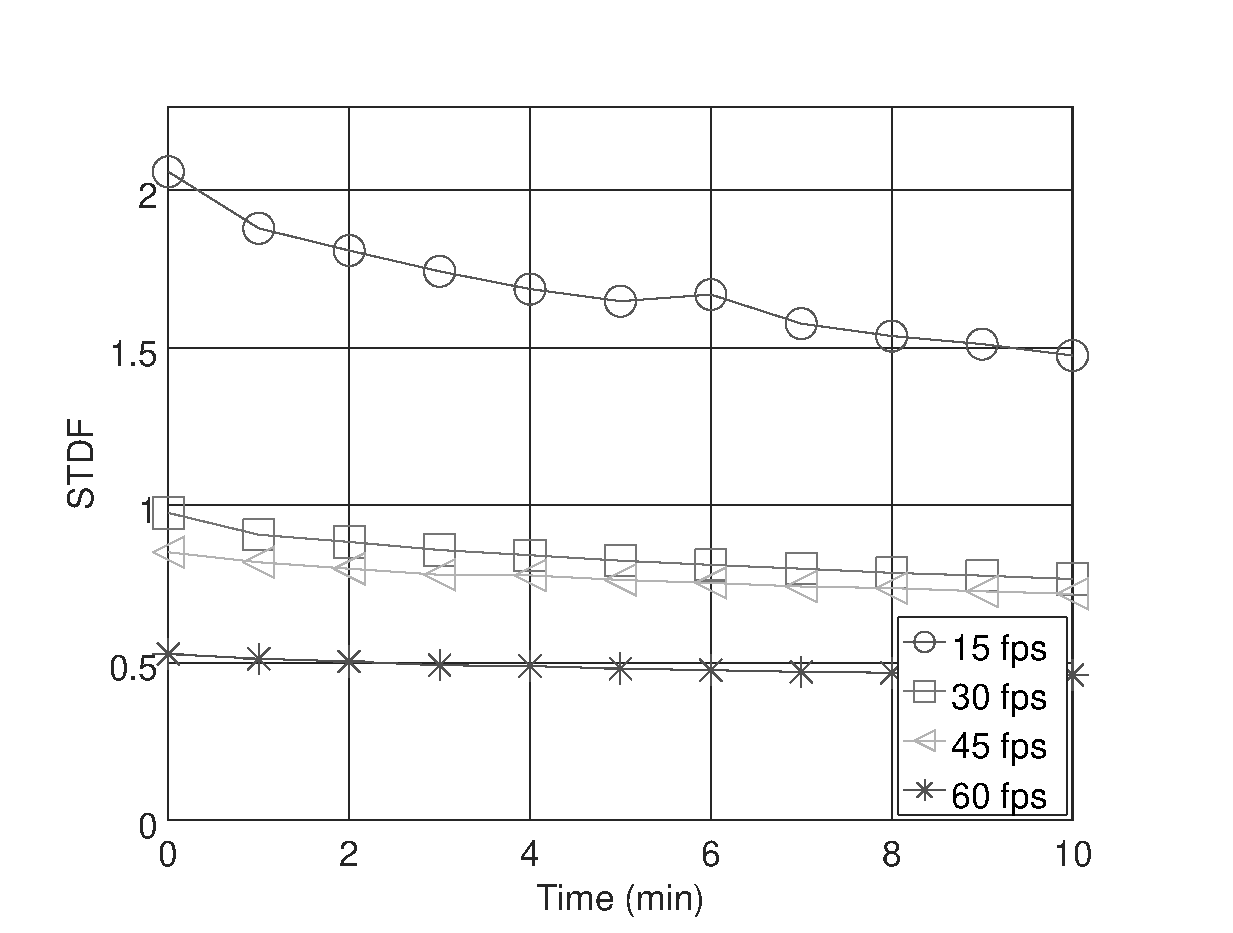
\includegraphics[width=\textwidth]{FPS_f11_rawSTDF.eps}
        \label{fig:stdfraw}
    \end{subfigure}
    ~ %add desired spacing between images, e. g. ~, \quad, \qquad, \hfill etc. 
      %(or a blank line to force the subfigure onto a new line)
    \begin{subfigure}{0.48\textwidth}
        \caption{Normalized $STDF$ index value.}
        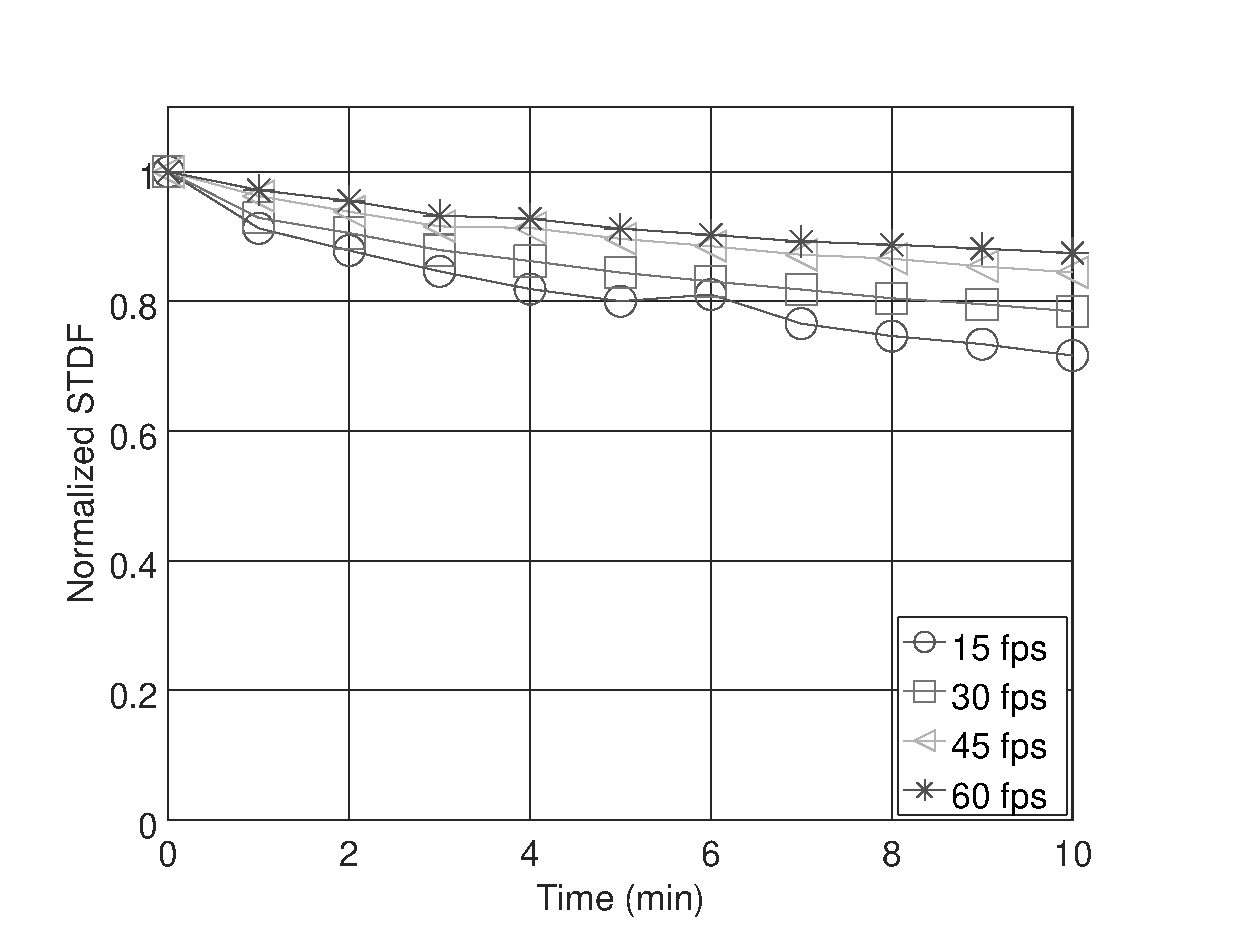
\includegraphics[width=\textwidth]{FPS_f11_norm1STDF.eps}
        \label{fig:stdfnorm}
    \end{subfigure}
    \caption{$STDF$ index anaysis.}\label{fig:STDFtest1}
\end{figure}
The Figure \ref{fig:stdfraw} shows the behavior $STDF(t)$ index, in each time $t$, 
to 4 different sampling frequencies. Remembering that this index uses filtered 
information of datapack, so that your frequency
band is between $F_s/4$ and $F_s/2$ Hz, of similar way of $AVD(t)$ index but with
different order filter, as seen in Section \ref{sec:stdf}.
This index shows monotone decreasing behavior in time, where we observe 
a different behavior across time to each different sampling frequency;
so that, the value of the index in each time of curve decreases in proportion with 
the grow of sampling frequency. By other side,
the Figure \ref{fig:stdfnorm} shows a normalized version of $STDF(t)$ index;
being the unit, the maximum value of curves; thus,
It is easy to see that exist a considerable difference between the maximum excursion 
of the curves with the use of sampling frequency; so, It is possible to observe a 
grow of the maximum excursion with the grow of the sampling frequency.


\subsection{Result of test 2}
\label{subsec:resulttest2}


\section{Analysis results} 
\label{sec:analysisresults}

\subsection{Analysis of results: test 1}
\label{subsec:analysistest1}
In the results of ink drying process test, seen in Section \ref{subsec:resulttest1},
we can observe in the Figure \ref{fig:MEANtest1}, that the index shows a relation 
between the value of curve and the sampling frequency of datapack. 
How is known \cite{Nothdurft:05}, the temporal speckle mean index is related to 
the observed illumination level in the surface of study material.
Thus, we can conclude that the level of illumination perceived by the camera decrease
with the increment of sampling frequency. 
This is because that the exposition time is modified, see Section \ref{subsec:expositiontime}, 
with the alteration of sampling frequency, 
so that less lighting is used to take the picture and consequently the 
temporal speckle mean index decrease in  your value.
The modification of exposition time also affect other indexes, 
how can it be seen in the Figures \ref{fig:AVDtest1}, \ref{fig:STDtest1} and  \ref{fig:STDFtest1}, 
where these indexes decrease your values in concordance with the decrease of exposition time.
Other way in that  the sampling frequency affect the values of indexes,
It is that it limits the band of signal frequency analyzed; for example,
a sampling frequency $F_s$ causes that the analyzed signal frequency band will be between $0 Hz$ and $F_s/2~Hz$.
Thus, in this context we have an index as $MEAN(t)$ that use information at  $0~Hz$ only, 
the index $STD(t)$ that use information between $\langle \left. 0, F_s/2 \right ] Hz$, 
and be other side we have indexes as the $AVD(t)$ and the $STDF(t)$ index, that use information of half frequency band, 
this is between $\left [ F_s/4, F_s/2 \right ] Hz$.
In the comparison between $STD(t)$ vs  $\{$ $STDF(t)$ and $AVD(t)$ $\}$, 
we can observe how the half part  use of frequency band causes the decrease of curves values, 
but considerably good values in the maximum excursion of the curve. By other side,
in the case of ink drying process, the use of complete frequency band, 
It returns low values of maximum excursion in the curves. 
The importance of excursion in this test,
 It is due the necessity of to have significant differences en the values of two states,
when the sample start or end the ink drying process.



%%%%%%%%%%%%%%%%%%%%%%%%%%%%%%%%%%%%%%%%%%%%%%%%%%%%%%%%%%%%%%%%%%%%%%%%%%%%%%%%%%%%%%%%%
%%%%%%%%%%%%%%%%%%%%%%%%%%%%%%%%%%%%%%%%%%%%%%%%%%%%%%%%%%%%%%%%%%%%%%%%%%%%%%%%%%%%%%%%%
\section{Conclusion} 

In this work were presented comparisons of behavior of three dynamic speckle indexes
subject to different values of sampling frequency, thus we concluded that:
It is important to know to choose an appropriate sampling frequency, 
being recommendable to use the minimal sampling frequency possible to get an acceptable maximum excursion,
so that the phenomenon under study to be in the analyzed frequency band.
Finally, 
we show that the digitization  of speckle signal imply a restriction of frequency 
band of signal and consequently this affect the result of an speckle analysis.

\section{Acknowledgment}
We wish to acknowledge the partial financial support for this study provided by the $CAPES$ 
scholarship
$PNPD$ Program, $FAPEMIG$ and $CNPQ$.

%----------------------------------------------------------------------------------------
%	REFERENCE LIST
%----------------------------------------------------------------------------------------
\section{Bibliography}
\bibliography{report}   %>>>> bibliography data in report.bib
\bibliographystyle{spiebib}   %>>>> makes bibtex use spiebib.bst


%----------------------------------------------------------------------------------------

\end{document} 


